\documentclass{llncs}

\usepackage{cite}
\usepackage{xspace}
\usepackage{hyperref}
\usepackage{xcolor}
\usepackage{graphicx}

\newcommand{\jkind}{{\sc JKind}\xspace}
\newcommand{\pkind}{{\sc PKind}\xspace}
\newcommand{\jkindapi}{{\sc JKindApi}\xspace}
\newcommand{\lustre}{{\sc Lustre}\xspace}
\newcommand{\spear}{{\sc SpeAR}\xspace}
\newcommand{\simpal}{{\sc SIMPAL}\xspace}
\newcommand{\limp}{{\sc Limp}\xspace}
\newcommand{\agree}{{\sc AGREE}\xspace}
\newcommand{\gryphon}{{\sc Gryphon}\xspace}
%\newcommand{\internal}{{\it internal}\xspace}

\newcommand{\todo}[1]{{\color{red} #1}}

\renewcommand{\paragraph}[1]{\vspace{5pt}\noindent {\bf #1}}

\title{JKind}
\author{
  Andrew Gacek\inst{1} \and
  John Backes\inst{2} \and
  Mike Whalen\inst{3} \and
  Lucas Wagner\inst{2} \and
  Elaheh Ghassabani\inst{3}}
\institute{
  Rockwell Collins \\
%  \email{andrew.gacek@gmail.com}, \email{lucas.wagner@rockwellcollins.com}
  \and
  Amazon Web Services \\
%  \email{john.backes@gmail.com}
  \and
  University of Minnesota
%  \email{ghass013@umn.edu}, \email{mwwhalen@umn.edu}
}

\begin{document}
\maketitle

\begin{abstract}
  \jkind is an open-source industrial model checker developed by
  Rockwell Collins and the University of Minnesota. We have developed
  \jkind as the back-end for various user-facing industrial
  applications. This paper describes the features \jkind, specifically
  focusing on these features inspired by industrial application.
\end{abstract}

\section{Introduction}

\jkind is an
open-source\footnote{\url{https://github.com/agacek/jkind}} industrial
infinite-state inductive model checker for safety properties. Models
and properties in \jkind are specified in \lustre
\cite{halbwachs1991ieee}, a synchronous data-flow language, using the
theories of linear real and integer arithmetic. \jkind uses
SMT-solvers to prove and falsify multiple properties in parallel.

A distinguishing characteristic of \jkind is its focus on the quality
of results. For a proven property, \jkind provides an inductive
validity core which traces the property back to individual model
elements. For a falsified property, \jkind provides options for
simplifying and generalizing the counterexample in order to highlight
what is causing the property to fail. In industrial applications, we
have found this additional quality of the results to be at least as
important as the primary results.

Another important characteristic of \jkind is that is it designed,
from the start, to be a library which sits underneath user-facing
applications. Written in Java, \jkind runs on all major platforms and
is easily compiled into other Java applications. While \jkind can use
the SMT-solvers {\sc Z3}, {\sc Yices 1}, {\sc Yices 2}, {\sc CVC4}, ,
and {\sc MathSAT}, it is also bundled with the Java-based {\sc
  SMTInterpol}. This means that applications can call out to \jkind
without requiring any other solvers to be natively installed. In
practice, we have found this to be indispensable for deploying
user-facing applications that are powered by model checking.

\section{Functionality and Main Features}

\begin{figure}
  \begin{center}
    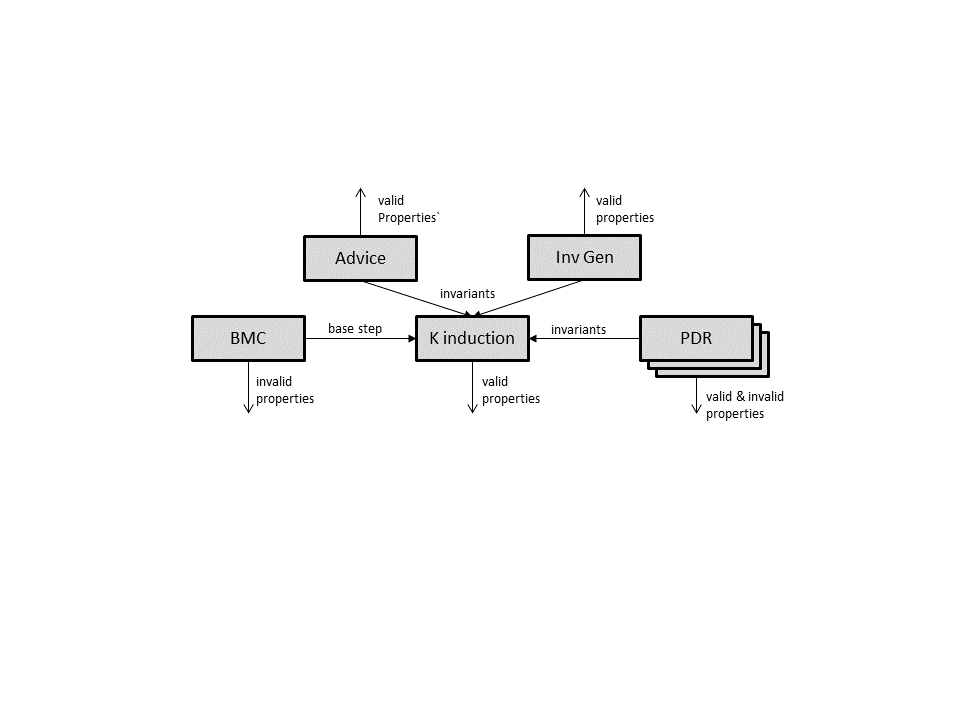
\includegraphics[scale=0.7]{engines.png}
  \end{center}
  \vspace{-2em}
  \caption{\jkind engine architecture}
  \vspace{-1em}
  \label{fig:engines}
\end{figure}

\jkind is structured as several parallel engines that coordinate to
prove properties, mimicking the design of \pkind
\cite{kahsai2011pdmc}. Some engines are directly responsible for
proving properties, others aid that effort by generating invariants,
and still others are reserved for post-processing of proof or
counterexample results. Each engine can be enabled or disabled
separately based on the user's needs. The core architecture of the
solving engines in \jkind is shown in Figure~\ref{fig:engines}.
Although displayed as point-to-point connections, information between
engines is actually broadcast so any engine pick the information it
wants.

The post-processing engines are greatest difference between \jkind
and more traditional model checkers. In industrial application, the
{\em quality} of an answer is just as important as the answer itself.
For example, more than knowing a property is true, we want to know
{\em why} it is true. We want to trace the property back to the model
and see which portions were exercised. This type of coverage and
traceability information is often required for certification of safety
critical systems.

% For completeness we describe each engine here, but we devote more
% space to the novel and distinguishing engines.

\paragraph{Bounded Model Checking (BMC).} The BMC engine performs a
standard iterative unrolling of the transition relation to find
counterexamples and to serve as the base case of $k$-induction. The
BMC engine guarantees that any counterexample it finds is minimal in
length.

\paragraph{$k$-induction.} The $k$-induction engine performs the
inductive step of $k$-induction, possibly using invariants generated by
other engines.

\paragraph{Invariant Generation.} The invariant generation engine uses
a template-based invariant generation technique \cite{kahsai2012nfm}
using its own $k$-induction loop.

\paragraph{Property Directed Reachability (PDR).} The PDR engine
performs property directed reachability \cite{een2011fmcad} using the
implicit abstraction technique \cite{cimatti2014tacas}. Unlike BMC and
$k$-induction, each property is handled separately by a different PDR
sub-engine. Invariants generated as a side-product of PDR are shared
with the $k$-induction process.

\paragraph{Inductive Validity Cores (IVC).} For a proven property, an
inductive validity core is a (hopefully small) subset of \lustre
equations from the input model for which the property still holds
\cite{ghassabani2016fse}. It indicates which portion of the model is
relevant to the proof of the property. The IVC engine uses a heuristic
algorithm to efficiently produce nearly minimal inductive validity
cores. As a side-product, the IVC algorithm also minimizes the set of
invariants used to prove a property and reports back this reduced set.

\paragraph{Advice.} The advice engine is used to save and re-use
results between runs of \jkind. When enabled, a set of invariant from a
previous run of \jkind, so called {\em advice}, is read in and
(hopefully) re-verified. Because advice is re-verified, it does not
need to be completely accurate. In particular, advice from a previous
run of \jkind can be used on a model even if that model is further
modified. Pieces of advice that successfully re-verify are used as
invariants while those that do not are discarded.

\paragraph{Smoothing.} Counterexamples generated from BMC and PDR are
not always easily understood, so as an optional post-processing step
we smooth counterexamples to minimize the number of changes to the
input variables. The smoothing engine uses a {\sc MaxSat} query over
the original BMC-style unrolling of the transition relation combined
with weighted assertions that each input variable does not change on
each step. The {\sc MaxSat} query therefore tries (as best as
possible) to hold all inputs constant while still falsifying the
original property. This engine is only available with solvers that
support {\sc MaxSat} such as Yices and Z3.

\paragraph{Interval Generalization.} Another post-processing step
available for counterexamples is to perform interval generalization
where individual values in a counterexample are replaced by intervals
that still falsify the property. This analysis is done purely through
simulation, without using an SMT-solver. It is useful in showing
that, for example, the value of a variable on a given step only needs
to be positive and its particular value does not matter.

\section{Integration \& Applications}

\jkind is the back-end for a variety of user-facing applications. In
this section, we briefly highlight a few applications and how they
employ the features discussed previously. \jkind is open-source and
some of these applications are as well (\spear, \agree, \simpal) while
the rest are proprietary.

We wrote \jkind in Java which makes it multi-platform and very easy to
integrate into other Java applications. Moreover, we created the
\jkindapi package which contains utilities for creating \lustre
specifications, calling \jkind, processing \jkind results, graphically
displaying real-time results, and nicely formatting counterexamples.
Many of the applications in this section make heavy use of \jkindapi.


\paragraph{Specification and Analysis of Requirements (\spear).}
The Specification and Analysis of Requirements tool, \spear for short,
is a prototyping and analysis tool for requirements expressed in
formal notations. \spear captures requirements in a way that is backed
by the formal semantics of \lustre, which enables them to be analyzed
using model checking to ensure they are correct and consistent.

\spear uses \jkind to prove properties over requirements, and uses IVC
to create a traceability matrix between requirements and properties.
This quickly highlights unused requirements, over-constrained
properties, and other common problems. \spear also uses \jkind for
test case generation using the Unique First Cause criteria
\cite{whalen2006issta} by creating {\em trap properties}. Each trap
property is expected to be falsifiable, but in such a way that the
counterexample has exactly the desired properties for a given test
case. \spear uses smoothing in \jkind to ensure the resulting test
cases are simple and understandable.

% \spear's approach to requirements capture and analysis represents a
% more rigorous approach than is used in traditional requirements
% verification. Traditional approaches rely on manual inspections of
% requirements to ensure the stated behaviors are correct and free from
% conflict. On the other hand, \spear's approach relies on model checking
% driven analyses, powered by \jkind to exhaustively analyze a set of
% requirements with respect to its behaviors, identifying incorrect
% behaviors and conflicting requirements sets automatically. The result
% is a more thoroughly analyzed set of requirements to hand to system
% designers and software developers.

\paragraph{Assume Guarantee Reasoning Environment (\agree). }
\jkind is used as the default model checker for the Assume Guarantee
Reasoning Environment (\agree). \agree refers to both an embedded
language annex in the Architectural Analysis and Design Language
(AADL) and a plugin to the OSATE AADL Integrated Development
Environment that reasons about the annex. The purpose of \agree is to
model behavioral requirements of an embedded system using formal
assume guarantee contracts. The plugin generates Lustre specifications
that are checked by \jkind.

\agree makes use of multiple \jkind features including smoothing and
interval generalization to present clear counterexamples, IVC to show
requirements traceability, and counterexample generation to check
consistency of an AADL component's contract. \agree also uses \jkind
to generate various test cases for AADL models annotated with
behavioral contracts. The test case generator uses counterexamples (or
lack thereof) to demonstrate requirements coverage.

\paragraph{Static IMPerative AnaLyzer (\simpal).}
The Static IMPerative AnaLyzer (\simpal) is a tool for performing
compositional reasoning over software programs that utilize
preexisting software components. \simpal features a specification
language, called \limp, for modeling programs that utilize preexisting
components. \limp is a \lustre-like imperative language. It
provides control flow elements, global variables, and a syntax for
specifying preconditions, postconditions, and global variable interactions
of preexisting components.
\simpal translates \limp programs to an equivalent \lustre representation
which is passed to the \jkind model checking tool
to perform assume-guarantee reasoning, reachability, and viability
analyses. The feedback from these analyses is used to refine
the program to ensure the software functions as intended.

\paragraph{The \gryphon Framework.} The Rockwell Collins \gryphon
framework \cite{miller2010cacm} translates Simulink models to various
analysis tools for verification and testing. \gryphon uses the \lustre
language internally which was the originally motivation for \pkind
(and eventually \jkind) to accept \lustre. As \gryphon is the only
application in our list which does not directly integrate \jkind, it
does not specifically use any features of \jkind. Still, features like
smoothing and IVC have been successfully used in combination with
\gryphon to great effect.

\paragraph{State Machines.} A flight control groups at Rockwell
Collins develops state machines which manage flight modes of an
aircraft. These state machines often have few states, but many
possible transitions between states. There is a priority ordering to
resolve conflicts between transitions, but this can make it hard to
fully exercise the behavior of a state machine. The flight controls
group has developed a particular graphical representation to manage
this complexity.

We have developed a tool which formalizes these state machine models.
It translates the state machine to \lustre and uses \jkind to check
properties over the state machine. We use IVCs to show which
transitions of a state machine are covered by which properties. We
also use trap properties to generate test cases exercising
transitions. Here IVCs are used when a trap property is true which
means it failed to generate a test case. The IVC indicates which
transitions are blocking the transition we wish to exercise in the
test case. The tool presents all this information graphically to the
flight controls group.

\paragraph{MC/DC Test Case Generation.} The Engine-Indicating and
Crew-Alerting System (EICAS) group at Rockwell Collins develops
equations which determine which messages and alerts should be
delivered to pilots. Certification for this system requires extensive
test cases which must satisfy criteria such as the Modified
Condition/Decision Coverage (MC/DC) metric. We have developed a tool
which generates these tests by translating the EICAS equations into
\lustre and generating MC/DC trap properties in \jkind. Smoothing is
very important in this context as test cases need to be run on the
actual hardware where timing is not precisely controllable. Thus, test
cases with a minimum of changes to the inputs are ideal.

\paragraph{Model-based Fuzzing.} As part of an ongoing DARPA program,
Rockwell Collins is developing a tool for generating fuzz tests from
system models. This tool takes a \lustre description of a system and
uses \jkind to generate test cases which exercise different portions
of the model. Effective fuzz testing requires a huge number of test
cases which is not feasible to generate solely with a model checker.
Instead, this fuzzing tool uses interval generalization in \jkind to
generate generalized counterexamples which it then randomly samples at
high speed. In fact, research in this area has recently expanded
interval generalization to trapezoidal generalization which is
strictly more general, but still allows very fast random sampling.

\section{Discussion}

\paragraph{Related Work}
\jkind is one of a number of similar infinite-state inductive model
checkers including {\sc Kind 2}, \pkind, {\sc NuXmv}, and {\sc
  Zustre}. These tools each offer multi-engine solvers that utilize
both k-induction and some variant of IC3/PDR. In a recent
comparison~\cite{champion2016cav}, \jkind was the second most capable
solver in terms of the number of problems solved (behind {\sc Kind 2})
and had competitive performance across a large benchmark suite. The
most noticeable bottleneck in \jkind is the start-up time for the Java
Virtual Machine (JVM). This cost is insignificant for larger models
but causes decreased performance for benchmarks consisting of many
very small models.

% \paragraph{Simulation.} To help users and developers to understand
% \lustre specifications, \jkind can compile a \lustre specification
% into an Excel-based simulation. The simulation uses the formula and
% reference language of Excel to compute, in real-time, the output of the
% specification as inputs are entered and manipulated. This spreadsheet
% interface to the specification is satisfyingly capable and versatile.

\paragraph{Conclusion}
\jkind is similar to a number of other solvers that each solve
infinite state sequential analysis problems. Nevertheless, it has some
important features that distinguish it. First, a focus on quality of
feedback to users for both valid properties (using IVCs) and invalid
properties (using smoothing and counterexample generalization).
Second, it is supported across all major platforms and is
straightforward to port due to its implementation in Java. Third, it
is small, modular, and well-architected, allowing straightforward
extension with new engines. Fourth, it is open source with a liberal
distribution license (BSD), so it can be adapted for various purposes,
as demonstrated by the number of tools that have incorporated it.

\section{Acknowledgments}

The work presented here was sponsored by DARPA as part of the HACMS
program under contract FA8750-12-9-0179.

\bibliography{main}{}
\bibliographystyle{splncs03}

\end{document}




% Local Variables:
% TeX-master: "main.tex"
% End:

%  LocalWords:  BMC PDR IVC MaxSat Yices SpeAR SIMPAL Gryphon UI JVM
%  LocalWords:  JKindApi natively PKind IMPerative AnaLyzer IVCs IC
%  LocalWords:  postconditions EICAS DARPA HACMS NuXmv Zustre
%  LocalWords:  architected
